% Options for packages loaded elsewhere
\PassOptionsToPackage{unicode}{hyperref}
\PassOptionsToPackage{hyphens}{url}
%
\documentclass[
]{article}
\usepackage{amsmath,amssymb}
\usepackage{lmodern}
\usepackage{iftex}
\ifPDFTeX
  \usepackage[T1]{fontenc}
  \usepackage[utf8]{inputenc}
  \usepackage{textcomp} % provide euro and other symbols
\else % if luatex or xetex
  \usepackage{unicode-math}
  \defaultfontfeatures{Scale=MatchLowercase}
  \defaultfontfeatures[\rmfamily]{Ligatures=TeX,Scale=1}
\fi
% Use upquote if available, for straight quotes in verbatim environments
\IfFileExists{upquote.sty}{\usepackage{upquote}}{}
\IfFileExists{microtype.sty}{% use microtype if available
  \usepackage[]{microtype}
  \UseMicrotypeSet[protrusion]{basicmath} % disable protrusion for tt fonts
}{}
\makeatletter
\@ifundefined{KOMAClassName}{% if non-KOMA class
  \IfFileExists{parskip.sty}{%
    \usepackage{parskip}
  }{% else
    \setlength{\parindent}{0pt}
    \setlength{\parskip}{6pt plus 2pt minus 1pt}}
}{% if KOMA class
  \KOMAoptions{parskip=half}}
\makeatother
\usepackage{xcolor}
\IfFileExists{xurl.sty}{\usepackage{xurl}}{} % add URL line breaks if available
\IfFileExists{bookmark.sty}{\usepackage{bookmark}}{\usepackage{hyperref}}
\hypersetup{
  hidelinks,
  pdfcreator={LaTeX via pandoc}}
\urlstyle{same} % disable monospaced font for URLs
\usepackage[margin=1in]{geometry}
\usepackage[ruled,vlined,linesnumbered]{algorithm2e}
\usepackage{listings}
\lstset{breaklines=true,basicstyle=\ttfamily\small,columns=fullflexible,keepspaces=true,showstringspaces=false}
\newcommand{\passthrough}[1]{#1}
\lstset{defaultdialect=[5.3]Lua}
\lstset{defaultdialect=[x86masm]Assembler}
\usepackage{graphicx}
\makeatletter
\def\maxwidth{\ifdim\Gin@nat@width>\linewidth\linewidth\else\Gin@nat@width\fi}
\def\maxheight{\ifdim\Gin@nat@height>\textheight\textheight\else\Gin@nat@height\fi}
\makeatother
% Scale images if necessary, so that they will not overflow the page
% margins by default, and it is still possible to overwrite the defaults
% using explicit options in \includegraphics[width, height, ...]{}
\setkeys{Gin}{width=\maxwidth,height=\maxheight,keepaspectratio}
% Set default figure placement to htbp
\makeatletter
\def\fps@figure{htbp}
\makeatother
\setlength{\emergencystretch}{3em} % prevent overfull lines
\providecommand{\tightlist}{%
  \setlength{\itemsep}{0pt}\setlength{\parskip}{0pt}}
\setcounter{secnumdepth}{-\maxdimen} % remove section numbering
\ifLuaTeX
  \usepackage{selnolig}  % disable illegal ligatures
\fi

\author{}
\date{}

\begin{document}

\hypertarget{homework-1}{%
\section{Homework 1}\label{homework-1}}

\hypertarget{runtime-analysis}{%
\subsection{1. Runtime Analysis}\label{runtime-analysis}}

\begin{enumerate}
\def\labelenumi{(\alph{enumi})}
\tightlist
\item
  \(w = 5 \times 10^{-9}\)\\
  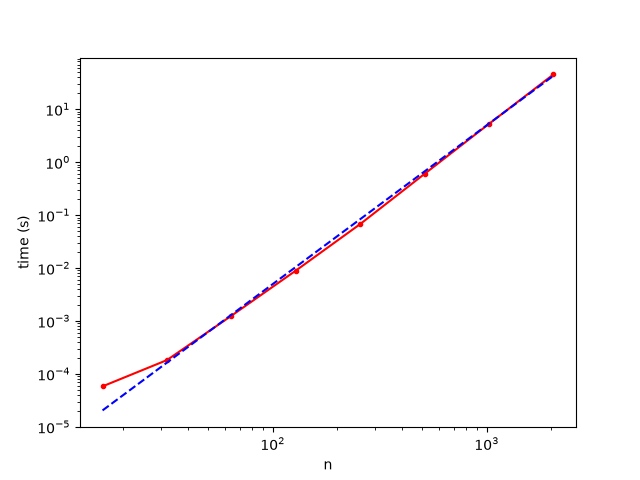
\includegraphics{./hw1_1_a_fig.png}
\item
\end{enumerate}

\begin{algorithm}[H]
\small
assert $a,b,c,n > 0$\;
assert $a,b,c \leq n$\tcp*{set bounds that a,b,c are at most n}
\BlankLine
\tcc{get the maximum numbers of each bill for the permutation}
$\text{max 3 buck} \gets \min(c,n/3)$\;
$\text{max 2 buck} \gets \min(b,n/2)$\;
$\text{max 1 buck} \gets \min(a,n)$\;
\BlankLine
\tcc{initialize the counter}
$\text{count} \gets 0$\;
\BlankLine
\For{the number of max 3 buck}{
    \For{the number of max 2 buck}{
        \If{$\begin{aligned}[t]
            &1.\ (3*\ \text{the number of 3 buck for each iteration}) > n\\
            &2.\ (2*\ \text{the number of 2 buck for each iteration}) > n\\
            &3.\ (n - (\\
            &\qquad (3*\ \text{the number of 3 buck for each iteration})\\
            &\qquad +\\
            &\qquad (2*\ \text{the number of 2 buck for each iteration})\\
            &\qquad ) > n\\
            &\quad )
        \end{aligned}$}{
            do nothing and move on\;
        }\Else{
            add 1 to count\;
        }
    }
}
\BlankLine
\Return count
\end{algorithm}

Proof:\\
Let \passthrough{\lstinline!a!} and \passthrough{\lstinline!b!} be the
number of 3-buck and 2-buck coins to be combined.\\
Let \passthrough{\lstinline!A!} be a 2D array that contains all sums of
permutations of \passthrough{\lstinline!a!} AND
\passthrough{\lstinline!b!} that those sums are always less than or
equal to \passthrough{\lstinline!n!}.\\
So, the number of possible permutations is \(a \times b\) and the
runtime is \(O(n^2)\).\\
If we add another condition that filters whether the value of each sum
in \passthrough{\lstinline!A!} subtracted by \passthrough{\lstinline!n!}
does not exceed the maximum number of 1-buck coin provided, we can
calculate all the possible permutation and how many the permutations
there are at the same time in \(n^2\) times.

Hence, the asymptotic coin choice algorithm can have time complexity of
\(O(n^2)\).

Runtime Analysis:\\
1. Variable initialization: the maximum number of coins we can combine
and counter \(O(1)\)

\begin{lstlisting}[language=Java]
int max_three_buck = Math.min(c, n/3);
int max_two_buck = Math.min(b,n/2);
int max_one_buck = Math.min(a,n);
int count = 0;
\end{lstlisting}

\begin{enumerate}
\def\labelenumi{\arabic{enumi}.}
\setcounter{enumi}{1}
\tightlist
\item
  Main Loop: \(O(n^2)\)
\end{enumerate}

\begin{enumerate}
\def\labelenumi{\arabic{enumi})}
\tightlist
\item
  iterate through the maximum numbers of three-buck and two-buck coin
  (O(n\^{}2))
\item
  eliminate the possible permutations that would go out of bounds from
  the counter\\
  2-1. if the given number of 3-buck coins worth more than n\\
  2-2. if the given number of 2-buck coins worth more than n\\
  2-3. if the given number of 3-AND-2-buck coins(permutation) worth more
  than n\\
  2-4. From the permutation without 2-1,2,3., if the left-over money is
  greater than the maximum number of 1-buck coin.\\
  2-5. Otherwise, put it in the counter.
\item
  Return the number of permutations (O(1))
\end{enumerate}

\begin{lstlisting}[language=Java]
for (int first = max_three_buck; first >= 0; first--){
    for (int second = max_two_buck; second >= 0; second--){
        if(3*first > n||2 * second > n || (3*first)+(2*second) > n || (n-(2*second+3*first)) > max_one_buck){
            continue;
        } else {
            count++;
        }
    }
}
\end{lstlisting}

\begin{enumerate}
\def\labelenumi{\arabic{enumi}.}
\setcounter{enumi}{2}
\tightlist
\item
  Return result: \(O(1)\)
\end{enumerate}

\begin{lstlisting}[language=Java]
return count;
\end{lstlisting}

Complete Runtime = \(O(1)\) + \(O(n^2)\) + \(O(1)\) = \(O(n^2)\)\\
Therefore, the runtime of this asymptotically faster algorithm for this
problem is \(O(n^2)\).\\
(c)\\
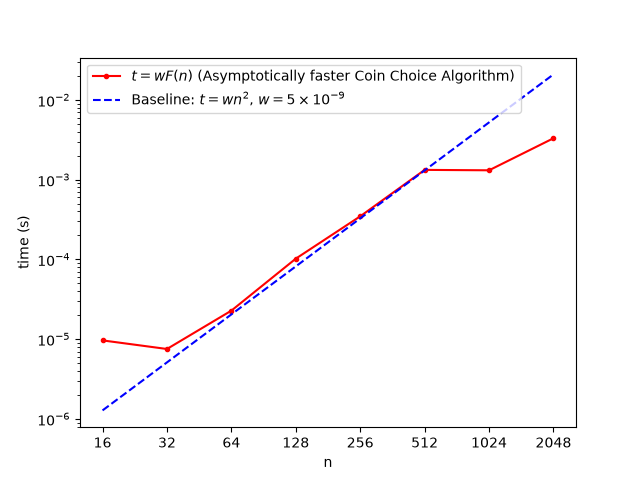
\includegraphics{./hw1_1_c_fig.png}\\
Initially, \passthrough{\lstinline!w!} value was \(5 \times 10^{-8}\) as
default. For part (a), I changed the exponent to \(-9\), which fits to
the original algorithm with time complexity of \(O(n^3)\). For the part
(c), I did not change \passthrough{\lstinline!w!} value and still able
to fit my asymptotically faster algorithm with time complexity of
\(O(n^2)\). Because \passthrough{\lstinline!w!} value is just an
adjustment parameter to make the comparison between the baseline
\(t=wn^2\) and my algorithm human-friendly and my hardware setup was not
changed, I did not have to change \passthrough{\lstinline!w!} value from
part (a). One problem I encountered was the data extraction. Since I
wrote the algorithm in Java and the original algorithm is in python, I
had to come up with an idea that I can put into the plot in python (I
don't know how to plot in Java so I had to extract data that can be read
cross-linguistically.)

\hypertarget{running-sum}{%
\subsection{2. Running Sum}\label{running-sum}}

\hypertarget{context}{%
\subsubsection{Context}\label{context}}

\begin{itemize}
\tightlist
\item
  Given arrays \(A\) and \(B\) (\(B\) with \(n\) elements),\\
  \[\begin{aligned}
  A[i] = B[i] + B[i+1] + B[i+2] + ... + B[i+r-1]\\
  \text{for all } i : 0 \leq  i \leq  n-r
  \end{aligned}
  \]
\item
  0-based indexing; \(i+r-1\) for upper bound.
\end{itemize}

\begin{enumerate}
\def\labelenumi{(\alph{enumi})}
\item
  The length of array \(A\) is \(n - r+1\). Because if the bound for
  \(i\) is \(0\leq i\leq n-r\), since it is inclusive and 0-based indexing, we
  need to add 1 to get the final array length and not loosing the last
  element of the array \(A\).
\item
  1st box: \passthrough{\lstinline!0!}\\
  2nd box: \passthrough{\lstinline!A.length!}\\
  3rd box: \passthrough{\lstinline!i!}\\
  4th box: \passthrough{\lstinline!i+r!}\\
  5th box: \passthrough{\lstinline!A[i] + B[j]!}
\item
  1st box: \passthrough{\lstinline!1!}\\
  2nd box: \passthrough{\lstinline!A.length!}\\
  3rd box: \passthrough{\lstinline!A[i-1] - B[i-1] + B[i+r-1]!}
\item
  Proof by Induction\\
  Prove \(A_i = \Sigma_{k=i}^{i+r-1} B_k\)
\end{enumerate}

\begin{enumerate}
\def\labelenumi{\arabic{enumi}.}
\item
  Base case: \(i=0, r=1\)\\
  \[
  \begin{array}{ll}
  A_0 = \Sigma_{k=0}^{0+1}B_k = \Sigma_{k=0}^{1}B_k = B_0+B_1\\\\
  \text{it holds!}
  \end{array}
  \]
\item
  Inductive Hypothesis: \\
  If \(A_i=\Sigma_{k=i}^{i+r-1}B_k\) holds, then
  \(A_i=\Sigma_{k=i}^{i+r-1}B_{k+1}\) holds.
\end{enumerate}

\[\begin{array}{ll}
A_i = B_i + B_{i+1} + ... + B_{i+r}\\
A_{i+1} = B_{i+1} + B_{i+2} + ... + B_{i+r}\\
A_{i+1}-A_i = -B_i + B_{i+r}\\
A_{i+1} = A_i-B_i+B_{i+r}
\end{array}
\]\\
The algorithm has a \passthrough{\lstinline!for!} loop of
\passthrough{\lstinline!O(n)!} time complexity that has the same
equation as \(A_{i+1}\). \(\square\)

\end{document}
